\documentclass[11pt]{article}
\usepackage[a4paper,margin=2cm]{geometry}
\usepackage{tikz}
\usepackage{amsmath}
\usetikzlibrary{decorations.pathreplacing,calligraphy,arrows.meta}

\setlength{\parindent}{0pt}\setlength{\parskip}{6pt}

\tikzset{
  real/.style={circle,draw=blue!55,fill=blue!12,minimum size=6mm,inner sep=0pt,font=\scriptsize},
  rand/.style={circle,draw=black!40,densely dashed,fill=black!5,minimum size=6mm,inner sep=0pt,
               font=\scriptsize,text=black!55},
  edge/.style={draw=black!40,line width=0.4pt},
}

\begin{document}

\begin{center}\Large\bfseries XMSS on small memory\end{center}

Valid for slots $[a,b]$, $R=b-a+1$. Only the $R$ leaves in $[a,b]$ are real WOTS keys; every other node
is a deterministic filler $\texttt{gen\_random\_node}$. We cut at $s=\texttt{split\_level}=\lceil\log_2 R\rceil/2$: the
\textbf{top} ($\approx\!\sqrt R$ nodes) is stored; the \textbf{bottom} is $\approx\!\sqrt R$
subtrees of $2^s$ leaves, indexed by $\texttt{subtree\_index}=\text{slot}\!\gg\!s$, of which only the signed
slot's one is (re)built and cached.

\begin{figure}[h]\centering
\resizebox{\linewidth}{!}{%
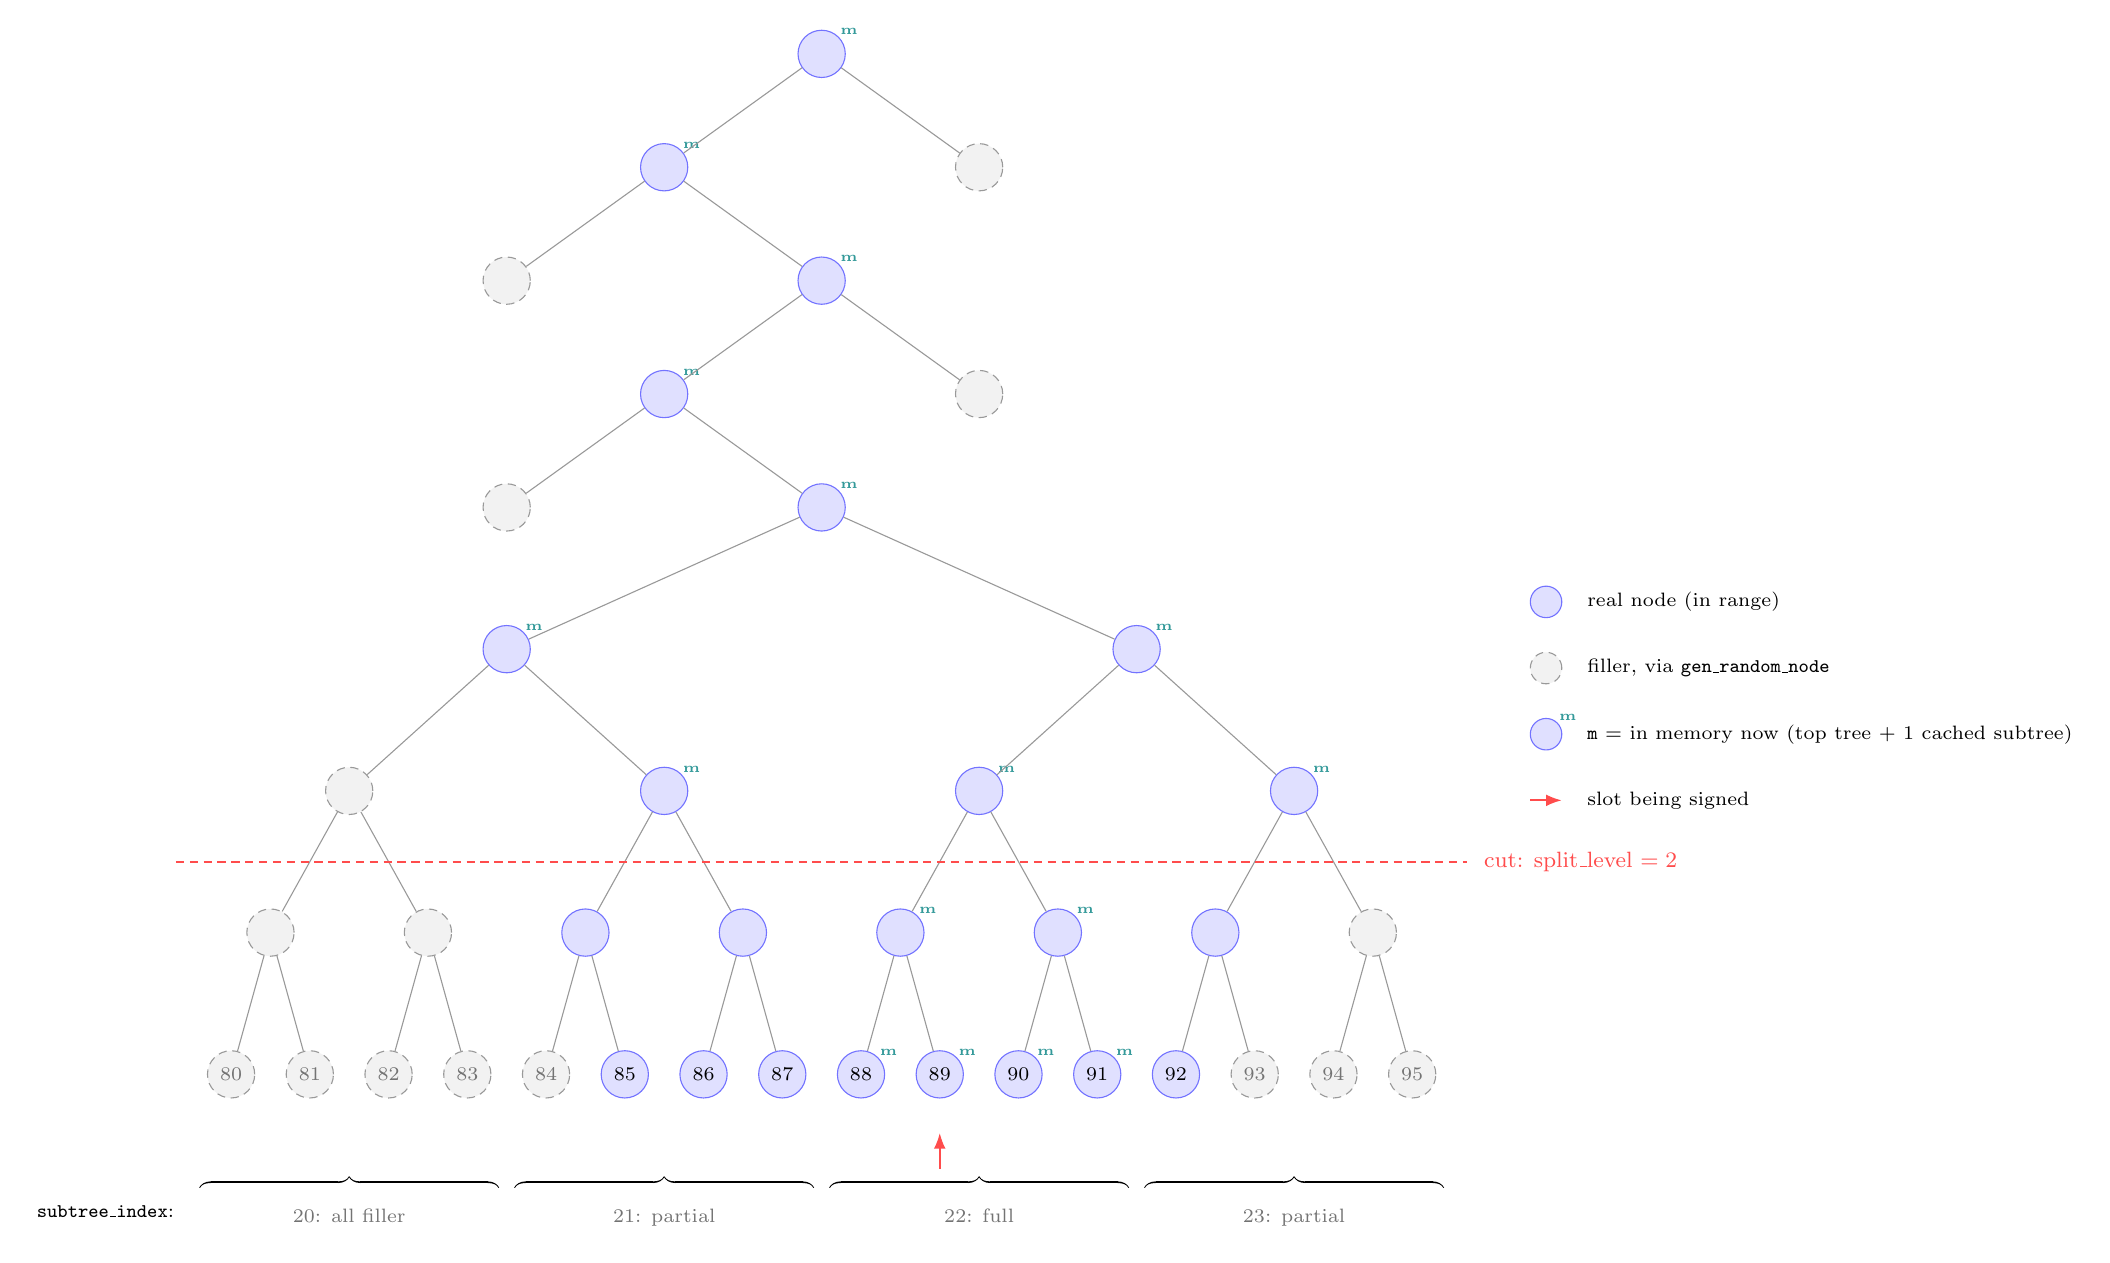
\begin{tikzpicture}[yscale=1.2]
  % bottom: the real region (8 leaves [85,92]) sits in a 16-leaf block (slots 80..95), levels 0..4.
  \foreach \i in {0,...,15}{\coordinate (lp\i) at (\i,0);}
  \foreach \i in {0,1,2,3,4,13,14,15}{\node[rand] (a\i) at (lp\i){\the\numexpr80+\i\relax};}
  \foreach \i in {5,6,7,8,9,10,11,12}{\node[real] (a\i) at (lp\i){\the\numexpr80+\i\relax};}
  \foreach \i in {0,...,7}{\coordinate (mp\i) at (2*\i+0.5,1.5);}
  \foreach \i in {0,1,7}{\node[rand] (b\i) at (mp\i){};}
  \foreach \i in {2,3,4,5,6}{\node[real] (b\i) at (mp\i){};}
  \node[rand] (c0) at (1.5,3){}; \node[real] (c1) at (5.5,3){};
  \node[real] (c2) at (9.5,3){};  \node[real] (c3) at (13.5,3){};
  \node[real] (d0) at (3.5,4.5){}; \node[real] (d1) at (11.5,4.5){};
  \node[real] (f0) at (7.5,6){};
  % top: a height-8 tree. Above the block the band is a single node; the real spine zigzags to the
  % root with a filler sibling at each level (its side follows the apex's index bits, not always left).
  \node[rand] (g4) at (3.5,6.0){};
  \node[real] (p5) at (5.5,7.2){};   \node[rand] (g5) at (9.5,7.2){};
  \node[real] (p6) at (7.5,8.4){};   \node[rand] (g6) at (3.5,8.4){};
  \node[real] (p7) at (5.5,9.6){};   \node[rand] (g7) at (9.5,9.6){};
  \node[real] (rt) at (7.5,10.8){};
  % small "m" badge = currently held in memory (top tree + the one cached subtree, here subtree 2).
  \foreach \n in {a8,a9,a10,a11,b4,b5,c1,c2,c3,d0,d1,f0,p5,p6,p7,rt}{
    \node[anchor=south west,font=\tiny\bfseries,text=teal!80,inner sep=0.4pt] at (\n.north east){m};
  }

  \foreach \i in {0,...,7}{\draw[edge] (b\i)--(a\the\numexpr2*\i\relax); \draw[edge] (b\i)--(a\the\numexpr2*\i+1\relax);}
  \foreach \i in {0,...,3}{\draw[edge] (c\i)--(b\the\numexpr2*\i\relax); \draw[edge] (c\i)--(b\the\numexpr2*\i+1\relax);}
  \draw[edge] (d0)--(c0); \draw[edge] (d0)--(c1); \draw[edge] (d1)--(c2); \draw[edge] (d1)--(c3);
  \draw[edge] (f0)--(d0); \draw[edge] (f0)--(d1);
  \draw[edge] (p5)--(f0); \draw[edge] (p5)--(g4);
  \draw[edge] (p6)--(p5); \draw[edge] (p6)--(g5);
  \draw[edge] (p7)--(p6); \draw[edge] (p7)--(g6);
  \draw[edge] (rt)--(p7); \draw[edge] (rt)--(g7);

  \draw[red!70,thick,densely dashed] (-0.7,2.25)--(15.7,2.25)
       node[right,font=\footnotesize,text=red!70]{\;cut: split\_level $=2$};

  % arrow at the slot currently being signed
  \draw[-{Latex[length=2mm]},red!70,line width=0.7pt] (9,-1.0) -- (9,-0.62);

  \node[anchor=east,font=\scriptsize] at (-0.6,-1.45){\texttt{subtree\_index}:};
  \foreach \k/\si/\lab in {0/20/{all filler},1/21/{partial},2/22/{full},3/23/{partial}}{
    \draw[decorate,decoration={calligraphic brace,amplitude=4pt},black!55,line width=0.6pt]
      (4*\k-0.4,-1.2) -- (4*\k+3.4,-1.2) node[midway,below=4pt,font=\scriptsize]{$\si$: \lab};
  }

  % legend
  \node[real,minimum size=4mm] at (16.7,5.0){};
  \node[anchor=west,font=\scriptsize] at (17.1,5.0){real node (in range)};
  \node[rand,minimum size=4mm] at (16.7,4.3){};
  \node[anchor=west,font=\scriptsize] at (17.1,4.3){filler, via $\texttt{gen\_random\_node}$};
  \node[real,minimum size=4mm] (Lm) at (16.7,3.6){};
  \node[anchor=south west,font=\tiny\bfseries,text=teal!80,inner sep=0.4pt] at (Lm.north east){m};
  \node[anchor=west,font=\scriptsize] at (17.1,3.6){\texttt{m} $=$ in memory now (top tree $+$ 1 cached subtree)};
  \draw[-{Latex[length=2mm]},red!70,line width=0.7pt] (16.5,2.9)--(16.9,2.9);
  \node[anchor=west,font=\scriptsize] at (17.1,2.9){slot being signed};
\end{tikzpicture}}
\caption{Example: signing slot 89 of $[a,b]=[85,92]$ ($R=8$, $s=2$) in an XMSS of lifetime $2^8$}
\end{figure}

\end{document}
